\documentclass[1p]{elsarticle_modified}
%\bibliographystyle{elsarticle-num}

%\usepackage[colorlinks]{hyperref}
%\usepackage{abbrmath_seonhwa} %\Abb, \Ascr, \Acal ,\Abf, \Afrak
\usepackage{amsfonts}
\usepackage{amssymb}
\usepackage{amsmath}
\usepackage{amsthm}
\usepackage{scalefnt}
\usepackage{amsbsy}
\usepackage{kotex}
\usepackage{caption}
\usepackage{subfig}
\usepackage{color}
\usepackage{graphicx}
\usepackage{xcolor} %% white, black, red, green, blue, cyan, magenta, yellow
\usepackage{float}
\usepackage{setspace}
\usepackage{hyperref}

\usepackage{tikz}
\usetikzlibrary{arrows}

\usepackage{multirow}
\usepackage{array} % fixed length table
\usepackage{hhline}

%%%%%%%%%%%%%%%%%%%%%
\makeatletter
\renewcommand*\env@matrix[1][\arraystretch]{%
	\edef\arraystretch{#1}%
	\hskip -\arraycolsep
	\let\@ifnextchar\new@ifnextchar
	\array{*\c@MaxMatrixCols c}}
\makeatother %https://tex.stackexchange.com/questions/14071/how-can-i-increase-the-line-spacing-in-a-matrix
%%%%%%%%%%%%%%%

\usepackage[normalem]{ulem}

\newcommand{\msout}[1]{\ifmmode\text{\sout{\ensuremath{#1}}}\else\sout{#1}\fi}
%SOURCE: \msout is \stkout macro in https://tex.stackexchange.com/questions/20609/strikeout-in-math-mode

\newcommand{\cancel}[1]{
	\ifmmode
	{\color{red}\msout{#1}}
	\else
	{\color{red}\sout{#1}}
	\fi
}

\newcommand{\add}[1]{
	{\color{blue}\uwave{#1}}
}

\newcommand{\replace}[2]{
	\ifmmode
	{\color{red}\msout{#1}}{\color{blue}\uwave{#2}}
	\else
	{\color{red}\sout{#1}}{\color{blue}\uwave{#2}}
	\fi
}

\newcommand{\Sol}{\mathcal{S}} %segment
\newcommand{\D}{D} %diagram
\newcommand{\A}{\mathcal{A}} %arc


%%%%%%%%%%%%%%%%%%%%%%%%%%%%%5 test

\def\sl{\operatorname{\textup{SL}}(2,\Cbb)}
\def\psl{\operatorname{\textup{PSL}}(2,\Cbb)}
\def\quan{\mkern 1mu \triangleright \mkern 1mu}

\theoremstyle{definition}
\newtheorem{thm}{Theorem}[section]
\newtheorem{prop}[thm]{Proposition}
\newtheorem{lem}[thm]{Lemma}
\newtheorem{ques}[thm]{Question}
\newtheorem{cor}[thm]{Corollary}
\newtheorem{defn}[thm]{Definition}
\newtheorem{exam}[thm]{Example}
\newtheorem{rmk}[thm]{Remark}
\newtheorem{alg}[thm]{Algorithm}

\newcommand{\I}{\sqrt{-1}}
\begin{document}

%\begin{frontmatter}
%
%\title{Boundary parabolic representations of knots up to 8 crossings}
%
%%% Group authors per affiliation:
%\author{Yunhi Cho} 
%\address{Department of Mathematics, University of Seoul, Seoul, Korea}
%\ead{yhcho@uos.ac.kr}
%
%
%\author{Seonhwa Kim} %\fnref{s_kim}}
%\address{Center for Geometry and Physics, Institute for Basic Science, Pohang, 37673, Korea}
%\ead{ryeona17@ibs.re.kr}
%
%\author{Hyuk Kim}
%\address{Department of Mathematical Sciences, Seoul National University, Seoul 08826, Korea}
%\ead{hyukkim@snu.ac.kr}
%
%\author{Seokbeom Yoon}
%\address{Department of Mathematical Sciences, Seoul National University, Seoul, 08826,  Korea}
%\ead{sbyoon15@snu.ac.kr}
%
%\begin{abstract}
%We find all boundary parabolic representation of knots up to 8 crossings.
%
%\end{abstract}
%\begin{keyword}
%    \MSC[2010] 57M25 
%\end{keyword}
%
%\end{frontmatter}

%\linenumbers
%\tableofcontents
%
\newcommand\colored[1]{\textcolor{white}{\rule[-0.35ex]{0.8em}{1.4ex}}\kern-0.8em\color{red} #1}%
%\newcommand\colored[1]{\textcolor{white}{ #1}\kern-2.17ex	\textcolor{white}{ #1}\kern-1.81ex	\textcolor{white}{ #1}\kern-2.15ex\color{red}#1	}

{\Large $\underline{12n_{0750}~(K12n_{0750})}$}

\setlength{\tabcolsep}{10pt}
\renewcommand{\arraystretch}{1.6}
\vspace{1cm}\begin{tabular}{m{100pt}>{\centering\arraybackslash}m{274pt}}
\multirow{5}{120pt}{
	\centering
	\includegraphics[width=112pt]{../../../GIT/diagram.site/Diagrams/png/2839_12n_0750.png}\\
\ \ \ A knot diagram\footnotemark}&
\allowdisplaybreaks
\textbf{Linearized knot diagam} \\
\cline{2-2}
 &
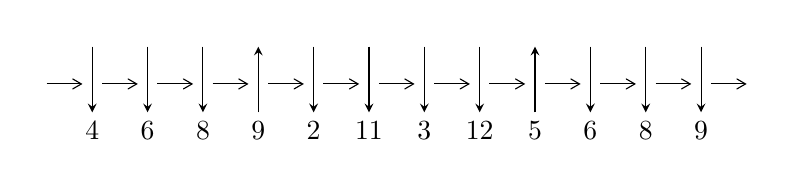
\begin{tikzpicture}[x=20pt, y=17pt]
	% nodes
	\node (C0) at (0, 0) {};
	\node (C1) at (1, 0) {};
	\node (C1U) at (1, +1) {};
	\node (C1D) at (1, -1) {4};

	\node (C2) at (2, 0) {};
	\node (C2U) at (2, +1) {};
	\node (C2D) at (2, -1) {6};

	\node (C3) at (3, 0) {};
	\node (C3U) at (3, +1) {};
	\node (C3D) at (3, -1) {8};

	\node (C4) at (4, 0) {};
	\node (C4U) at (4, +1) {};
	\node (C4D) at (4, -1) {9};

	\node (C5) at (5, 0) {};
	\node (C5U) at (5, +1) {};
	\node (C5D) at (5, -1) {2};

	\node (C6) at (6, 0) {};
	\node (C6U) at (6, +1) {};
	\node (C6D) at (6, -1) {11};

	\node (C7) at (7, 0) {};
	\node (C7U) at (7, +1) {};
	\node (C7D) at (7, -1) {3};

	\node (C8) at (8, 0) {};
	\node (C8U) at (8, +1) {};
	\node (C8D) at (8, -1) {12};

	\node (C9) at (9, 0) {};
	\node (C9U) at (9, +1) {};
	\node (C9D) at (9, -1) {5};

	\node (C10) at (10, 0) {};
	\node (C10U) at (10, +1) {};
	\node (C10D) at (10, -1) {6};

	\node (C11) at (11, 0) {};
	\node (C11U) at (11, +1) {};
	\node (C11D) at (11, -1) {8};

	\node (C12) at (12, 0) {};
	\node (C12U) at (12, +1) {};
	\node (C12D) at (12, -1) {9};
	\node (C13) at (13, 0) {};

	% arrows
	\draw[->,>={angle 60}]
	(C0) edge (C1) (C1) edge (C2) (C2) edge (C3) (C3) edge (C4) (C4) edge (C5) (C5) edge (C6) (C6) edge (C7) (C7) edge (C8) (C8) edge (C9) (C9) edge (C10) (C10) edge (C11) (C11) edge (C12) (C12) edge (C13) ;	\draw[->,>=stealth]
	(C1U) edge (C1D) (C2U) edge (C2D) (C3U) edge (C3D) (C4D) edge (C4U) (C5U) edge (C5D) (C6U) edge (C6D) (C7U) edge (C7D) (C8U) edge (C8D) (C9D) edge (C9U) (C10U) edge (C10D) (C11U) edge (C11D) (C12U) edge (C12D) ;
	\end{tikzpicture} \\
\hhline{~~} \\& 
\textbf{Solving Sequence} \\ \cline{2-2} 
 &
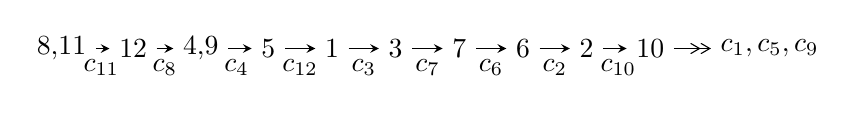
\begin{tikzpicture}[x=23pt, y=7pt]
	% node
	\node (A0) at (-1/8, 0) {8,11};
	\node (A1) at (1, 0) {12};
	\node (A2) at (33/16, 0) {4,9};
	\node (A3) at (25/8, 0) {5};
	\node (A4) at (33/8, 0) {1};
	\node (A5) at (41/8, 0) {3};
	\node (A6) at (49/8, 0) {7};
	\node (A7) at (57/8, 0) {6};
	\node (A8) at (65/8, 0) {2};
	\node (A9) at (73/8, 0) {10};
	\node (C1) at (1/2, -1) {$c_{11}$};
	\node (C2) at (3/2, -1) {$c_{8}$};
	\node (C3) at (21/8, -1) {$c_{4}$};
	\node (C4) at (29/8, -1) {$c_{12}$};
	\node (C5) at (37/8, -1) {$c_{3}$};
	\node (C6) at (45/8, -1) {$c_{7}$};
	\node (C7) at (53/8, -1) {$c_{6}$};
	\node (C8) at (61/8, -1) {$c_{2}$};
	\node (C9) at (69/8, -1) {$c_{10}$};
	\node (A10) at (11, 0) {$c_{1},c_{5},c_{9}$};

	% edge
	\draw[->,>=stealth]	
	(A0) edge (A1) (A1) edge (A2) (A2) edge (A3) (A3) edge (A4) (A4) edge (A5) (A5) edge (A6) (A6) edge (A7) (A7) edge (A8) (A8) edge (A9) ;
	\draw[->>,>={angle 60}]	
	(A9) edge (A10);
\end{tikzpicture} \\ 

\end{tabular} \\

\footnotetext{
The image of knot diagram is generated by the software ``\textbf{Draw programme}" developed by Andrew Bartholomew(\url{http://www.layer8.co.uk/maths/draw/index.htm\#Running-draw}), where we modified some parts for our purpose(\url{https://github.com/CATsTAILs/LinksPainter}).
}\phantom \\ \newline 
\centering \textbf{Ideals for irreducible components\footnotemark of $X_{\text{par}}$} 
 
\begin{align*}
I^u_{1}&=\langle 
-2 u^5-10 u^4-15 u^3+13 u^2+5 b+45 u+19,\;-7 u^5-25 u^4-20 u^3+43 u^2+15 a+85 u+24,\\
\phantom{I^u_{1}}&\phantom{= \langle  }u^6+4 u^5+5 u^4-4 u^3-16 u^2-12 u-3\rangle \\
I^u_{2}&=\langle 
-2 u^2+b+u+2,\;a- u,\;u^3- u^2+1\rangle \\
I^u_{3}&=\langle 
-2 u^2 a- u^2+b+a+u,\;a^2+a u- u^2+u-1,\;u^3- u^2+1\rangle \\
I^u_{4}&=\langle 
2 u^3- u^2+3 b-1,\;u^3+4 u^2+3 a+9 u+4,\;u^4+3 u^3+5 u^2+u-1\rangle \\
I^u_{5}&=\langle 
u^2+b-3,\;-3 u^3+4 u^2+5 a+7 u-10,\;u^4-3 u^3+u^2+5 u-5\rangle \\
I^u_{6}&=\langle 
-3 a u+2 b+6 a+u,\;4 a^2+2 a u-6 a-5 u+3,\;u^2- u+2\rangle \\
I^u_{7}&=\langle 
b^2+b-1,\;a+1,\;u+1\rangle \\
\\
I^v_{1}&=\langle 
a,\;b+v-2,\;v^2-3 v+1\rangle \\
I^v_{2}&=\langle 
a,\;b-1,\;v-1\rangle \\
\end{align*}
\raggedright * 9 irreducible components of $\dim_{\mathbb{C}}=0$, with total 32 representations.\\
\footnotetext{All coefficients of polynomials are rational numbers. But the coefficients are sometimes approximated in decimal forms when there is not enough margin.}
\newpage
\renewcommand{\arraystretch}{1}
\centering \section*{I. $I^u_{1}= \langle -2 u^5-10 u^4+\cdots+5 b+19,\;-7 u^5-25 u^4+\cdots+15 a+24,\;u^6+4 u^5+5 u^4-4 u^3-16 u^2-12 u-3 \rangle$}
\flushleft \textbf{(i) Arc colorings}\\
\begin{tabular}{m{7pt} m{180pt} m{7pt} m{180pt} }
\flushright $a_{8}=$&$\begin{pmatrix}0\\u\end{pmatrix}$ \\
\flushright $a_{11}=$&$\begin{pmatrix}1\\0\end{pmatrix}$ \\
\flushright $a_{12}=$&$\begin{pmatrix}1\\u^2\end{pmatrix}$ \\
\flushright $a_{4}=$&$\begin{pmatrix}\frac{7}{15} u^5+\frac{5}{3} u^4+\cdots-\frac{17}{3} u-\frac{8}{5}\\\frac{2}{5} u^5+2 u^4+3 u^3-\frac{13}{5} u^2-9 u-\frac{19}{5}\end{pmatrix}$ \\
\flushright $a_{9}=$&$\begin{pmatrix}- u\\- u^3+u\end{pmatrix}$ \\
\flushright $a_{5}=$&$\begin{pmatrix}\frac{13}{15} u^5+\frac{8}{3} u^4+\cdots-\frac{29}{3} u-\frac{17}{5}\\\frac{7}{5} u^5+4 u^4+2 u^3-\frac{38}{5} u^2-11 u-\frac{19}{5}\end{pmatrix}$ \\
\flushright $a_{1}=$&$\begin{pmatrix}- u^2+1\\- u^4+2 u^2\end{pmatrix}$ \\
\flushright $a_{3}=$&$\begin{pmatrix}\frac{7}{15} u^5+\frac{5}{3} u^4+\cdots-\frac{17}{3} u-\frac{8}{5}\\\frac{3}{5} u^5+2 u^4+2 u^3-\frac{17}{5} u^2-8 u-\frac{16}{5}\end{pmatrix}$ \\
\flushright $a_{7}=$&$\begin{pmatrix}-\frac{4}{15} u^5-\frac{2}{3} u^4+\cdots+\frac{8}{3} u+\frac{6}{5}\\-\frac{1}{5} u^5- u^4- u^3+\frac{9}{5} u^2+4 u+\frac{7}{5}\end{pmatrix}$ \\
\flushright $a_{6}=$&$\begin{pmatrix}-\frac{7}{15} u^5-\frac{5}{3} u^4+\cdots+\frac{20}{3} u+\frac{13}{5}\\-\frac{1}{5} u^5- u^4- u^3+\frac{9}{5} u^2+4 u+\frac{7}{5}\end{pmatrix}$ \\
\flushright $a_{2}=$&$\begin{pmatrix}\frac{4}{15} u^5+\frac{2}{3} u^4+\cdots-\frac{8}{3} u-\frac{1}{5}\\\frac{4}{5} u^5+2 u^4+u^3-\frac{21}{5} u^2-7 u-\frac{13}{5}\end{pmatrix}$ \\
\flushright $a_{10}=$&$\begin{pmatrix}\frac{2}{15} u^5+\frac{1}{3} u^4+\cdots-\frac{1}{3} u+\frac{7}{5}\\-\frac{2}{5} u^5- u^4+\frac{8}{5} u^2+2 u+\frac{4}{5}\end{pmatrix}$\\&\end{tabular}
\flushleft \textbf{(ii) Obstruction class $= -1$}\\~\\
\flushleft \textbf{(iii) Cusp Shapes $= \frac{26}{5} u^5+18 u^4+16 u^3-\frac{154}{5} u^2-72 u-\frac{192}{5}$}\\~\\
\newpage\renewcommand{\arraystretch}{1}
\flushleft \textbf{(iv) u-Polynomials at the component}\newline \\
\begin{tabular}{m{50pt}|m{274pt}}
Crossings & \hspace{64pt}u-Polynomials at each crossing \\
\hline $$\begin{aligned}c_{1},c_{3},c_{6}\\c_{7},c_{10}\end{aligned}$$&$\begin{aligned}
&u^6-2 u^5+5 u^4+2 u^3-4 u^2-2 u-1
\end{aligned}$\\
\hline $$\begin{aligned}c_{2},c_{5},c_{8}\\c_{11},c_{12}\end{aligned}$$&$\begin{aligned}
&u^6+4 u^5+5 u^4-4 u^3-16 u^2-12 u-3
\end{aligned}$\\
\hline $$\begin{aligned}c_{4},c_{9}\end{aligned}$$&$\begin{aligned}
&u^6+2 u^5- u^4-2 u^3-2 u+1
\end{aligned}$\\
\hline
\end{tabular}\\~\\
\newpage\renewcommand{\arraystretch}{1}
\flushleft \textbf{(v) Riley Polynomials at the component}\newline \\
\begin{tabular}{m{50pt}|m{274pt}}
Crossings & \hspace{64pt}Riley Polynomials at each crossing \\
\hline $$\begin{aligned}c_{1},c_{3},c_{6}\\c_{7},c_{10}\end{aligned}$$&$\begin{aligned}
&y^6+6 y^5+25 y^4-54 y^3+14 y^2+4 y+1
\end{aligned}$\\
\hline $$\begin{aligned}c_{2},c_{5},c_{8}\\c_{11},c_{12}\end{aligned}$$&$\begin{aligned}
&y^6-6 y^5+25 y^4-86 y^3+130 y^2-48 y+9
\end{aligned}$\\
\hline $$\begin{aligned}c_{4},c_{9}\end{aligned}$$&$\begin{aligned}
&y^6-6 y^5+9 y^4+6 y^3-10 y^2-4 y+1
\end{aligned}$\\
\hline
\end{tabular}\\~\\
\newpage\flushleft \textbf{(vi) Complex Volumes and Cusp Shapes}
$$\begin{array}{c|c|c}  
\text{Solutions to }I^u_{1}& \I (\text{vol} + \sqrt{-1}CS) & \text{Cusp shape}\\
 \hline 
\begin{aligned}
u &= -0.510485 + 0.215723 I \\
a &= \phantom{-}0.602418 - 0.514537 I \\
b &= \phantom{-}0.055837 - 1.062600 I\end{aligned}
 & -0.807577 + 0.909082 I & -9.16175 - 7.66066 I \\ \hline\begin{aligned}
u &= -0.510485 - 0.215723 I \\
a &= \phantom{-}0.602418 + 0.514537 I \\
b &= \phantom{-}0.055837 + 1.062600 I\end{aligned}
 & -0.807577 - 0.909082 I & -9.16175 + 7.66066 I \\ \hline\begin{aligned}
u &= \phantom{-}1.52560\phantom{ +0.000000I} \\
a &= \phantom{-}0.702173\phantom{ +0.000000I} \\
b &= \phantom{-}1.21012\phantom{ +0.000000I}\end{aligned}
 & -11.8129\phantom{ +0.000000I} & -22.6370\phantom{ +0.000000I} \\ \hline\begin{aligned}
u &= -1.70948\phantom{ +0.000000I} \\
a &= \phantom{-}0.469310\phantom{ +0.000000I} \\
b &= \phantom{-}0.240689\phantom{ +0.000000I}\end{aligned}
 & -9.43829\phantom{ +0.000000I} & -7.45040\phantom{ +0.000000I} \\ \hline\begin{aligned}
u &= -1.39757 + 1.33871 I \\
a &= -1.188160 + 0.447062 I \\
b &= \phantom{-}3.21876 + 4.79537 I\end{aligned}
 & \phantom{-}13.9006 + 10.5245 I & -7.79449 - 4.24029 I \\ \hline\begin{aligned}
u &= -1.39757 - 1.33871 I \\
a &= -1.188160 - 0.447062 I \\
b &= \phantom{-}3.21876 - 4.79537 I\end{aligned}
 & \phantom{-}13.9006 - 10.5245 I & -7.79449 + 4.24029 I\\
 \hline 
 \end{array}$$\newpage\newpage\renewcommand{\arraystretch}{1}
\centering \section*{II. $I^u_{2}= \langle -2 u^2+b+u+2,\;a- u,\;u^3- u^2+1 \rangle$}
\flushleft \textbf{(i) Arc colorings}\\
\begin{tabular}{m{7pt} m{180pt} m{7pt} m{180pt} }
\flushright $a_{8}=$&$\begin{pmatrix}0\\u\end{pmatrix}$ \\
\flushright $a_{11}=$&$\begin{pmatrix}1\\0\end{pmatrix}$ \\
\flushright $a_{12}=$&$\begin{pmatrix}1\\u^2\end{pmatrix}$ \\
\flushright $a_{4}=$&$\begin{pmatrix}u\\2 u^2- u-2\end{pmatrix}$ \\
\flushright $a_{9}=$&$\begin{pmatrix}- u\\- u^2+u+1\end{pmatrix}$ \\
\flushright $a_{5}=$&$\begin{pmatrix}-1\\0\end{pmatrix}$ \\
\flushright $a_{1}=$&$\begin{pmatrix}- u^2+1\\u^2+u+1\end{pmatrix}$ \\
\flushright $a_{3}=$&$\begin{pmatrix}u\\u^2- u-1\end{pmatrix}$ \\
\flushright $a_{7}=$&$\begin{pmatrix}u^2-1\\- u^2\end{pmatrix}$ \\
\flushright $a_{6}=$&$\begin{pmatrix}-1\\- u^2\end{pmatrix}$ \\
\flushright $a_{2}=$&$\begin{pmatrix}0\\- u\end{pmatrix}$ \\
\flushright $a_{10}=$&$\begin{pmatrix}- u^2+1\\- u^2+u+1\end{pmatrix}$\\&\end{tabular}
\flushleft \textbf{(ii) Obstruction class $= 1$}\\~\\
\flushleft \textbf{(iii) Cusp Shapes $= 8 u-12$}\\~\\
\newpage\renewcommand{\arraystretch}{1}
\flushleft \textbf{(iv) u-Polynomials at the component}\newline \\
\begin{tabular}{m{50pt}|m{274pt}}
Crossings & \hspace{64pt}u-Polynomials at each crossing \\
\hline $$\begin{aligned}c_{1},c_{3},c_{6}\end{aligned}$$&$\begin{aligned}
&u^3- u^2+2 u-1
\end{aligned}$\\
\hline $$\begin{aligned}c_{2},c_{8}\end{aligned}$$&$\begin{aligned}
&u^3+u^2-1
\end{aligned}$\\
\hline $$\begin{aligned}c_{4}\end{aligned}$$&$\begin{aligned}
&u^3+3 u^2+2 u-1
\end{aligned}$\\
\hline $$\begin{aligned}c_{5},c_{11},c_{12}\end{aligned}$$&$\begin{aligned}
&u^3- u^2+1
\end{aligned}$\\
\hline $$\begin{aligned}c_{7},c_{10}\end{aligned}$$&$\begin{aligned}
&u^3+u^2+2 u+1
\end{aligned}$\\
\hline $$\begin{aligned}c_{9}\end{aligned}$$&$\begin{aligned}
&u^3-3 u^2+2 u+1
\end{aligned}$\\
\hline
\end{tabular}\\~\\
\newpage\renewcommand{\arraystretch}{1}
\flushleft \textbf{(v) Riley Polynomials at the component}\newline \\
\begin{tabular}{m{50pt}|m{274pt}}
Crossings & \hspace{64pt}Riley Polynomials at each crossing \\
\hline $$\begin{aligned}c_{1},c_{3},c_{6}\\c_{7},c_{10}\end{aligned}$$&$\begin{aligned}
&y^3+3 y^2+2 y-1
\end{aligned}$\\
\hline $$\begin{aligned}c_{2},c_{5},c_{8}\\c_{11},c_{12}\end{aligned}$$&$\begin{aligned}
&y^3- y^2+2 y-1
\end{aligned}$\\
\hline $$\begin{aligned}c_{4},c_{9}\end{aligned}$$&$\begin{aligned}
&y^3-5 y^2+10 y-1
\end{aligned}$\\
\hline
\end{tabular}\\~\\
\newpage\flushleft \textbf{(vi) Complex Volumes and Cusp Shapes}
$$\begin{array}{c|c|c}  
\text{Solutions to }I^u_{2}& \I (\text{vol} + \sqrt{-1}CS) & \text{Cusp shape}\\
 \hline 
\begin{aligned}
u &= \phantom{-}0.877439 + 0.744862 I \\
a &= \phantom{-}0.877439 + 0.744862 I \\
b &= -2.44728 + 1.86942 I\end{aligned}
 & \phantom{-}6.04826 - 5.65624 I & -4.98049 + 5.95889 I \\ \hline\begin{aligned}
u &= \phantom{-}0.877439 - 0.744862 I \\
a &= \phantom{-}0.877439 - 0.744862 I \\
b &= -2.44728 - 1.86942 I\end{aligned}
 & \phantom{-}6.04826 + 5.65624 I & -4.98049 - 5.95889 I \\ \hline\begin{aligned}
u &= -0.754878\phantom{ +0.000000I} \\
a &= -0.754878\phantom{ +0.000000I} \\
b &= -0.105442\phantom{ +0.000000I}\end{aligned}
 & -2.22691\phantom{ +0.000000I} & -18.0390\phantom{ +0.000000I}\\
 \hline 
 \end{array}$$\newpage\newpage\renewcommand{\arraystretch}{1}
\centering \section*{III. $I^u_{3}= \langle -2 u^2 a- u^2+b+a+u,\;a^2+a u- u^2+u-1,\;u^3- u^2+1 \rangle$}
\flushleft \textbf{(i) Arc colorings}\\
\begin{tabular}{m{7pt} m{180pt} m{7pt} m{180pt} }
\flushright $a_{8}=$&$\begin{pmatrix}0\\u\end{pmatrix}$ \\
\flushright $a_{11}=$&$\begin{pmatrix}1\\0\end{pmatrix}$ \\
\flushright $a_{12}=$&$\begin{pmatrix}1\\u^2\end{pmatrix}$ \\
\flushright $a_{4}=$&$\begin{pmatrix}a\\2 u^2 a+u^2- a- u\end{pmatrix}$ \\
\flushright $a_{9}=$&$\begin{pmatrix}- u\\- u^2+u+1\end{pmatrix}$ \\
\flushright $a_{5}=$&$\begin{pmatrix}u^2 a- a u- u\\1\end{pmatrix}$ \\
\flushright $a_{1}=$&$\begin{pmatrix}- u^2+1\\u^2+u+1\end{pmatrix}$ \\
\flushright $a_{3}=$&$\begin{pmatrix}a\\u^2 a+u^2- a- u\end{pmatrix}$ \\
\flushright $a_{7}=$&$\begin{pmatrix}- u^2 a+u-1\\a u\end{pmatrix}$ \\
\flushright $a_{6}=$&$\begin{pmatrix}- u^2 a+a u+u-1\\a u\end{pmatrix}$ \\
\flushright $a_{2}=$&$\begin{pmatrix}- u^2+u\\u^2- a- u\end{pmatrix}$ \\
\flushright $a_{10}=$&$\begin{pmatrix}- u^2 a+2 a u- u^2+u\\u^2 a- u^2- a+u\end{pmatrix}$\\&\end{tabular}
\flushleft \textbf{(ii) Obstruction class $= -1$}\\~\\
\flushleft \textbf{(iii) Cusp Shapes $= 8 u-18$}\\~\\
\newpage\renewcommand{\arraystretch}{1}
\flushleft \textbf{(iv) u-Polynomials at the component}\newline \\
\begin{tabular}{m{50pt}|m{274pt}}
Crossings & \hspace{64pt}u-Polynomials at each crossing \\
\hline $$\begin{aligned}c_{1},c_{3},c_{6}\\c_{7},c_{10}\end{aligned}$$&$\begin{aligned}
&u^6+u^5+2 u^4-4 u^2+2 u-1
\end{aligned}$\\
\hline $$\begin{aligned}c_{2},c_{5},c_{8}\\c_{11},c_{12}\end{aligned}$$&$\begin{aligned}
&(u^3- u^2+1)^2
\end{aligned}$\\
\hline $$\begin{aligned}c_{4},c_{9}\end{aligned}$$&$\begin{aligned}
&u^6+3 u^5-4 u^3+6 u^2+14 u+5
\end{aligned}$\\
\hline
\end{tabular}\\~\\
\newpage\renewcommand{\arraystretch}{1}
\flushleft \textbf{(v) Riley Polynomials at the component}\newline \\
\begin{tabular}{m{50pt}|m{274pt}}
Crossings & \hspace{64pt}Riley Polynomials at each crossing \\
\hline $$\begin{aligned}c_{1},c_{3},c_{6}\\c_{7},c_{10}\end{aligned}$$&$\begin{aligned}
&y^6+3 y^5-4 y^4-22 y^3+12 y^2+4 y+1
\end{aligned}$\\
\hline $$\begin{aligned}c_{2},c_{5},c_{8}\\c_{11},c_{12}\end{aligned}$$&$\begin{aligned}
&(y^3- y^2+2 y-1)^2
\end{aligned}$\\
\hline $$\begin{aligned}c_{4},c_{9}\end{aligned}$$&$\begin{aligned}
&y^6-9 y^5+36 y^4-90 y^3+148 y^2-136 y+25
\end{aligned}$\\
\hline
\end{tabular}\\~\\
\newpage\flushleft \textbf{(vi) Complex Volumes and Cusp Shapes}
$$\begin{array}{c|c|c}  
\text{Solutions to }I^u_{3}& \I (\text{vol} + \sqrt{-1}CS) & \text{Cusp shape}\\
 \hline 
\begin{aligned}
u &= \phantom{-}0.877439 + 0.744862 I \\
a &= -1.26420 - 0.91095 I \\
b &= \phantom{-}2.43950 - 2.22359 I\end{aligned}
 & \phantom{-}4.40332 - 5.65624 I & -10.98049 + 5.95889 I \\ \hline\begin{aligned}
u &= \phantom{-}0.877439 + 0.744862 I \\
a &= \phantom{-}0.386757 + 0.166085 I \\
b &= -1.31694 + 1.47873 I\end{aligned}
 & \phantom{-}4.40332 - 5.65624 I & -10.98049 + 5.95889 I \\ \hline\begin{aligned}
u &= \phantom{-}0.877439 - 0.744862 I \\
a &= -1.26420 + 0.91095 I \\
b &= \phantom{-}2.43950 + 2.22359 I\end{aligned}
 & \phantom{-}4.40332 + 5.65624 I & -10.98049 - 5.95889 I \\ \hline\begin{aligned}
u &= \phantom{-}0.877439 - 0.744862 I \\
a &= \phantom{-}0.386757 - 0.166085 I \\
b &= -1.31694 - 1.47873 I\end{aligned}
 & \phantom{-}4.40332 + 5.65624 I & -10.98049 - 5.95889 I \\ \hline\begin{aligned}
u &= -0.754878\phantom{ +0.000000I} \\
a &= -1.19329\phantom{ +0.000000I} \\
b &= \phantom{-}1.15804\phantom{ +0.000000I}\end{aligned}
 & -3.87184\phantom{ +0.000000I} & -24.0390\phantom{ +0.000000I} \\ \hline\begin{aligned}
u &= -0.754878\phantom{ +0.000000I} \\
a &= \phantom{-}1.94816\phantom{ +0.000000I} \\
b &= \phantom{-}1.59684\phantom{ +0.000000I}\end{aligned}
 & -3.87184\phantom{ +0.000000I} & -24.0390\phantom{ +0.000000I}\\
 \hline 
 \end{array}$$\newpage\newpage\renewcommand{\arraystretch}{1}
\centering \section*{IV. $I^u_{4}= \langle 2 u^3- u^2+3 b-1,\;u^3+4 u^2+3 a+9 u+4,\;u^4+3 u^3+5 u^2+u-1 \rangle$}
\flushleft \textbf{(i) Arc colorings}\\
\begin{tabular}{m{7pt} m{180pt} m{7pt} m{180pt} }
\flushright $a_{8}=$&$\begin{pmatrix}0\\u\end{pmatrix}$ \\
\flushright $a_{11}=$&$\begin{pmatrix}1\\0\end{pmatrix}$ \\
\flushright $a_{12}=$&$\begin{pmatrix}1\\u^2\end{pmatrix}$ \\
\flushright $a_{4}=$&$\begin{pmatrix}-\frac{1}{3} u^3-\frac{4}{3} u^2-3 u-\frac{4}{3}\\-\frac{2}{3} u^3+\frac{1}{3} u^2+\frac{1}{3}\end{pmatrix}$ \\
\flushright $a_{9}=$&$\begin{pmatrix}- u\\- u^3+u\end{pmatrix}$ \\
\flushright $a_{5}=$&$\begin{pmatrix}- u^3-3 u^2-4 u-1\\\frac{4}{3} u^3+\frac{4}{3} u^2+\frac{1}{3}\end{pmatrix}$ \\
\flushright $a_{1}=$&$\begin{pmatrix}- u^2+1\\3 u^3+7 u^2+u-1\end{pmatrix}$ \\
\flushright $a_{3}=$&$\begin{pmatrix}-\frac{1}{3} u^3-\frac{4}{3} u^2-3 u-\frac{4}{3}\\-\frac{1}{3} u^3-\frac{1}{3} u^2+\frac{2}{3}\end{pmatrix}$ \\
\flushright $a_{7}=$&$\begin{pmatrix}\frac{1}{3} u^3+\frac{1}{3} u^2+2 u+\frac{4}{3}\\\frac{1}{3} u^3+\frac{4}{3} u^2+u-\frac{2}{3}\end{pmatrix}$ \\
\flushright $a_{6}=$&$\begin{pmatrix}\frac{2}{3} u^3+\frac{5}{3} u^2+3 u+\frac{2}{3}\\\frac{1}{3} u^3+\frac{4}{3} u^2+u-\frac{2}{3}\end{pmatrix}$ \\
\flushright $a_{2}=$&$\begin{pmatrix}-\frac{1}{3} u^3-\frac{4}{3} u^2-2 u-\frac{1}{3}\\\frac{1}{3} u^3+\frac{4}{3} u^2+\frac{1}{3}\end{pmatrix}$ \\
\flushright $a_{10}=$&$\begin{pmatrix}u+1\\\frac{4}{3} u^3+\frac{7}{3} u^2+u-\frac{2}{3}\end{pmatrix}$\\&\end{tabular}
\flushleft \textbf{(ii) Obstruction class $= -1$}\\~\\
\flushleft \textbf{(iii) Cusp Shapes $= -7$}\\~\\
\newpage\renewcommand{\arraystretch}{1}
\flushleft \textbf{(iv) u-Polynomials at the component}\newline \\
\begin{tabular}{m{50pt}|m{274pt}}
Crossings & \hspace{64pt}u-Polynomials at each crossing \\
\hline $$\begin{aligned}c_{1},c_{3},c_{6}\\c_{7},c_{10}\end{aligned}$$&$\begin{aligned}
&u^4+2 u^3+8 u^2+7 u+1
\end{aligned}$\\
\hline $$\begin{aligned}c_{2},c_{5},c_{8}\\c_{11},c_{12}\end{aligned}$$&$\begin{aligned}
&u^4+3 u^3+5 u^2+u-1
\end{aligned}$\\
\hline $$\begin{aligned}c_{4},c_{9}\end{aligned}$$&$\begin{aligned}
&(u^2- u-1)^2
\end{aligned}$\\
\hline
\end{tabular}\\~\\
\newpage\renewcommand{\arraystretch}{1}
\flushleft \textbf{(v) Riley Polynomials at the component}\newline \\
\begin{tabular}{m{50pt}|m{274pt}}
Crossings & \hspace{64pt}Riley Polynomials at each crossing \\
\hline $$\begin{aligned}c_{1},c_{3},c_{6}\\c_{7},c_{10}\end{aligned}$$&$\begin{aligned}
&y^4+12 y^3+38 y^2-33 y+1
\end{aligned}$\\
\hline $$\begin{aligned}c_{2},c_{5},c_{8}\\c_{11},c_{12}\end{aligned}$$&$\begin{aligned}
&y^4+y^3+17 y^2-11 y+1
\end{aligned}$\\
\hline $$\begin{aligned}c_{4},c_{9}\end{aligned}$$&$\begin{aligned}
&(y^2-3 y+1)^2
\end{aligned}$\\
\hline
\end{tabular}\\~\\
\newpage\flushleft \textbf{(vi) Complex Volumes and Cusp Shapes}
$$\begin{array}{c|c|c}  
\text{Solutions to }I^u_{4}& \I (\text{vol} + \sqrt{-1}CS) & \text{Cusp shape}\\
 \hline 
\begin{aligned}
u &= -0.713039\phantom{ +0.000000I} \\
a &= \phantom{-}0.248726\phantom{ +0.000000I} \\
b &= \phantom{-}0.744493\phantom{ +0.000000I}\end{aligned}
 & -1.31595\phantom{ +0.000000I} & -7.00000\phantom{ +0.000000I} \\ \hline\begin{aligned}
u &= \phantom{-}0.331073\phantom{ +0.000000I} \\
a &= -2.48479\phantom{ +0.000000I} \\
b &= \phantom{-}0.345677\phantom{ +0.000000I}\end{aligned}
 & -1.31595\phantom{ +0.000000I} & -7.00000\phantom{ +0.000000I} \\ \hline\begin{aligned}
u &= -1.30902 + 1.58825 I \\
a &= \phantom{-}1.118030 - 0.606658 I \\
b &= -5.04508 - 4.15810 I\end{aligned}
 & \phantom{-}14.4754\phantom{ +0.000000I} & -7.00000\phantom{ +0.000000I} \\ \hline\begin{aligned}
u &= -1.30902 - 1.58825 I \\
a &= \phantom{-}1.118030 + 0.606658 I \\
b &= -5.04508 + 4.15810 I\end{aligned}
 & \phantom{-}14.4754\phantom{ +0.000000I} & -7.00000\phantom{ +0.000000I}\\
 \hline 
 \end{array}$$\newpage\newpage\renewcommand{\arraystretch}{1}
\centering \section*{V. $I^u_{5}= \langle u^2+b-3,\;-3 u^3+4 u^2+5 a+7 u-10,\;u^4-3 u^3+u^2+5 u-5 \rangle$}
\flushleft \textbf{(i) Arc colorings}\\
\begin{tabular}{m{7pt} m{180pt} m{7pt} m{180pt} }
\flushright $a_{8}=$&$\begin{pmatrix}0\\u\end{pmatrix}$ \\
\flushright $a_{11}=$&$\begin{pmatrix}1\\0\end{pmatrix}$ \\
\flushright $a_{12}=$&$\begin{pmatrix}1\\u^2\end{pmatrix}$ \\
\flushright $a_{4}=$&$\begin{pmatrix}\frac{3}{5} u^3-\frac{4}{5} u^2-\frac{7}{5} u+2\\- u^2+3\end{pmatrix}$ \\
\flushright $a_{9}=$&$\begin{pmatrix}- u\\- u^3+u\end{pmatrix}$ \\
\flushright $a_{5}=$&$\begin{pmatrix}-\frac{7}{5} u^3+\frac{11}{5} u^2+\frac{8}{5} u-3\\-2 u^3+4 u^2+2 u-7\end{pmatrix}$ \\
\flushright $a_{1}=$&$\begin{pmatrix}- u^2+1\\-3 u^3+3 u^2+5 u-5\end{pmatrix}$ \\
\flushright $a_{3}=$&$\begin{pmatrix}\frac{3}{5} u^3-\frac{4}{5} u^2-\frac{7}{5} u+2\\- u^3+u^2+2 u-2\end{pmatrix}$ \\
\flushright $a_{7}=$&$\begin{pmatrix}-\frac{1}{5} u^3+\frac{3}{5} u^2+\frac{4}{5} u-2\\u^3-2 u^2- u+4\end{pmatrix}$ \\
\flushright $a_{6}=$&$\begin{pmatrix}\frac{4}{5} u^3-\frac{7}{5} u^2-\frac{1}{5} u+2\\u^3-2 u^2- u+4\end{pmatrix}$ \\
\flushright $a_{2}=$&$\begin{pmatrix}-\frac{1}{5} u^3-\frac{2}{5} u^2+\frac{4}{5} u-1\\- u^3+2 u-1\end{pmatrix}$ \\
\flushright $a_{10}=$&$\begin{pmatrix}-\frac{6}{5} u^3+\frac{8}{5} u^2+\frac{9}{5} u-3\\-2 u^3+3 u^2+3 u-6\end{pmatrix}$\\&\end{tabular}
\flushleft \textbf{(ii) Obstruction class $= 1$}\\~\\
\flushleft \textbf{(iii) Cusp Shapes $= -7$}\\~\\
\newpage\renewcommand{\arraystretch}{1}
\flushleft \textbf{(iv) u-Polynomials at the component}\newline \\
\begin{tabular}{m{50pt}|m{274pt}}
Crossings & \hspace{64pt}u-Polynomials at each crossing \\
\hline $$\begin{aligned}c_{1},c_{3},c_{6}\end{aligned}$$&$\begin{aligned}
&u^4+2 u^3+2 u^2+u-1
\end{aligned}$\\
\hline $$\begin{aligned}c_{2},c_{8}\end{aligned}$$&$\begin{aligned}
&u^4+3 u^3+u^2-5 u-5
\end{aligned}$\\
\hline $$\begin{aligned}c_{4}\end{aligned}$$&$\begin{aligned}
&(u^2- u-1)^2
\end{aligned}$\\
\hline $$\begin{aligned}c_{5},c_{11},c_{12}\end{aligned}$$&$\begin{aligned}
&u^4-3 u^3+u^2+5 u-5
\end{aligned}$\\
\hline $$\begin{aligned}c_{7},c_{10}\end{aligned}$$&$\begin{aligned}
&u^4-2 u^3+2 u^2- u-1
\end{aligned}$\\
\hline $$\begin{aligned}c_{9}\end{aligned}$$&$\begin{aligned}
&(u^2+u-1)^2
\end{aligned}$\\
\hline
\end{tabular}\\~\\
\newpage\renewcommand{\arraystretch}{1}
\flushleft \textbf{(v) Riley Polynomials at the component}\newline \\
\begin{tabular}{m{50pt}|m{274pt}}
Crossings & \hspace{64pt}Riley Polynomials at each crossing \\
\hline $$\begin{aligned}c_{1},c_{3},c_{6}\\c_{7},c_{10}\end{aligned}$$&$\begin{aligned}
&y^4-2 y^2-5 y+1
\end{aligned}$\\
\hline $$\begin{aligned}c_{2},c_{5},c_{8}\\c_{11},c_{12}\end{aligned}$$&$\begin{aligned}
&y^4-7 y^3+21 y^2-35 y+25
\end{aligned}$\\
\hline $$\begin{aligned}c_{4},c_{9}\end{aligned}$$&$\begin{aligned}
&(y^2-3 y+1)^2
\end{aligned}$\\
\hline
\end{tabular}\\~\\
\newpage\flushleft \textbf{(vi) Complex Volumes and Cusp Shapes}
$$\begin{array}{c|c|c}  
\text{Solutions to }I^u_{5}& \I (\text{vol} + \sqrt{-1}CS) & \text{Cusp shape}\\
 \hline 
\begin{aligned}
u &= -1.31651\phantom{ +0.000000I} \\
a &= \phantom{-}1.08748\phantom{ +0.000000I} \\
b &= \phantom{-}1.26680\phantom{ +0.000000I}\end{aligned}
 & -11.1856\phantom{ +0.000000I} & -7.00000\phantom{ +0.000000I} \\ \hline\begin{aligned}
u &= \phantom{-}1.30902 + 0.72287 I \\
a &= -0.670820 - 0.523074 I \\
b &= \phantom{-}1.80902 - 1.89250 I\end{aligned}
 & \phantom{-}4.60582\phantom{ +0.000000I} & -7.00000\phantom{ +0.000000I} \\ \hline\begin{aligned}
u &= \phantom{-}1.30902 - 0.72287 I \\
a &= -0.670820 + 0.523074 I \\
b &= \phantom{-}1.80902 + 1.89250 I\end{aligned}
 & \phantom{-}4.60582\phantom{ +0.000000I} & -7.00000\phantom{ +0.000000I} \\ \hline\begin{aligned}
u &= \phantom{-}1.69848\phantom{ +0.000000I} \\
a &= \phantom{-}0.254159\phantom{ +0.000000I} \\
b &= \phantom{-}0.115171\phantom{ +0.000000I}\end{aligned}
 & -11.1856\phantom{ +0.000000I} & -7.00000\phantom{ +0.000000I}\\
 \hline 
 \end{array}$$\newpage\newpage\renewcommand{\arraystretch}{1}
\centering \section*{VI. $I^u_{6}= \langle -3 a u+2 b+6 a+u,\;4 a^2+2 a u-6 a-5 u+3,\;u^2- u+2 \rangle$}
\flushleft \textbf{(i) Arc colorings}\\
\begin{tabular}{m{7pt} m{180pt} m{7pt} m{180pt} }
\flushright $a_{8}=$&$\begin{pmatrix}0\\u\end{pmatrix}$ \\
\flushright $a_{11}=$&$\begin{pmatrix}1\\0\end{pmatrix}$ \\
\flushright $a_{12}=$&$\begin{pmatrix}1\\u-2\end{pmatrix}$ \\
\flushright $a_{4}=$&$\begin{pmatrix}a\\\frac{3}{2} a u-3 a-\frac{1}{2} u\end{pmatrix}$ \\
\flushright $a_{9}=$&$\begin{pmatrix}- u\\2 u+2\end{pmatrix}$ \\
\flushright $a_{5}=$&$\begin{pmatrix}-\frac{1}{2} a u+\frac{1}{2} u+1\\\frac{3}{2} a u+a-\frac{1}{2} u-4\end{pmatrix}$ \\
\flushright $a_{1}=$&$\begin{pmatrix}- u+3\\5 u-6\end{pmatrix}$ \\
\flushright $a_{3}=$&$\begin{pmatrix}a\\\frac{1}{2} a u- a-\frac{1}{2} u\end{pmatrix}$ \\
\flushright $a_{7}=$&$\begin{pmatrix}a u+a+\frac{1}{2} u-\frac{5}{2}\\-\frac{1}{2} a u- a-\frac{1}{2} u+2\end{pmatrix}$ \\
\flushright $a_{6}=$&$\begin{pmatrix}\frac{1}{2} a u-\frac{1}{2}\\-\frac{1}{2} a u- a-\frac{1}{2} u+2\end{pmatrix}$ \\
\flushright $a_{2}=$&$\begin{pmatrix}-\frac{1}{2} u+\frac{1}{2}\\-\frac{1}{2} a u+a+\frac{3}{2} u-1\end{pmatrix}$ \\
\flushright $a_{10}=$&$\begin{pmatrix}- a-\frac{1}{2} u+\frac{1}{2}\\-\frac{1}{2} a u+3 a+\frac{1}{2} u\end{pmatrix}$\\&\end{tabular}
\flushleft \textbf{(ii) Obstruction class $= -1$}\\~\\
\flushleft \textbf{(iii) Cusp Shapes $= -7$}\\~\\
\newpage\renewcommand{\arraystretch}{1}
\flushleft \textbf{(iv) u-Polynomials at the component}\newline \\
\begin{tabular}{m{50pt}|m{274pt}}
Crossings & \hspace{64pt}u-Polynomials at each crossing \\
\hline $$\begin{aligned}c_{1},c_{3},c_{6}\\c_{7},c_{10}\end{aligned}$$&$\begin{aligned}
&u^4-3 u^3+8 u^2-13 u+11
\end{aligned}$\\
\hline $$\begin{aligned}c_{2},c_{5},c_{8}\\c_{11},c_{12}\end{aligned}$$&$\begin{aligned}
&(u^2- u+2)^2
\end{aligned}$\\
\hline $$\begin{aligned}c_{4},c_{9}\end{aligned}$$&$\begin{aligned}
&(u^2- u-1)^2
\end{aligned}$\\
\hline
\end{tabular}\\~\\
\newpage\renewcommand{\arraystretch}{1}
\flushleft \textbf{(v) Riley Polynomials at the component}\newline \\
\begin{tabular}{m{50pt}|m{274pt}}
Crossings & \hspace{64pt}Riley Polynomials at each crossing \\
\hline $$\begin{aligned}c_{1},c_{3},c_{6}\\c_{7},c_{10}\end{aligned}$$&$\begin{aligned}
&y^4+7 y^3+8 y^2+7 y+121
\end{aligned}$\\
\hline $$\begin{aligned}c_{2},c_{5},c_{8}\\c_{11},c_{12}\end{aligned}$$&$\begin{aligned}
&(y^2+3 y+4)^2
\end{aligned}$\\
\hline $$\begin{aligned}c_{4},c_{9}\end{aligned}$$&$\begin{aligned}
&(y^2-3 y+1)^2
\end{aligned}$\\
\hline
\end{tabular}\\~\\
\newpage\flushleft \textbf{(vi) Complex Volumes and Cusp Shapes}
$$\begin{array}{c|c|c}  
\text{Solutions to }I^u_{6}& \I (\text{vol} + \sqrt{-1}CS) & \text{Cusp shape}\\
 \hline 
\begin{aligned}
u &= \phantom{-}0.50000 + 1.32288 I \\
a &= -0.213525 - 1.070230 I \\
b &= \phantom{-}2.35410 + 1.32288 I\end{aligned}
 & \phantom{-}6.57974\phantom{ +0.000000I} & -7.00000\phantom{ +0.000000I} \\ \hline\begin{aligned}
u &= \phantom{-}0.50000 + 1.32288 I \\
a &= \phantom{-}1.46353 + 0.40879 I \\
b &= -4.35410 + 1.32288 I\end{aligned}
 & \phantom{-}6.57974\phantom{ +0.000000I} & -7.00000\phantom{ +0.000000I} \\ \hline\begin{aligned}
u &= \phantom{-}0.50000 - 1.32288 I \\
a &= -0.213525 + 1.070230 I \\
b &= \phantom{-}2.35410 - 1.32288 I\end{aligned}
 & \phantom{-}6.57974\phantom{ +0.000000I} & -7.00000\phantom{ +0.000000I} \\ \hline\begin{aligned}
u &= \phantom{-}0.50000 - 1.32288 I \\
a &= \phantom{-}1.46353 - 0.40879 I \\
b &= -4.35410 - 1.32288 I\end{aligned}
 & \phantom{-}6.57974\phantom{ +0.000000I} & -7.00000\phantom{ +0.000000I}\\
 \hline 
 \end{array}$$\newpage\newpage\renewcommand{\arraystretch}{1}
\centering \section*{VII. $I^u_{7}= \langle b^2+b-1,\;a+1,\;u+1 \rangle$}
\flushleft \textbf{(i) Arc colorings}\\
\begin{tabular}{m{7pt} m{180pt} m{7pt} m{180pt} }
\flushright $a_{8}=$&$\begin{pmatrix}0\\-1\end{pmatrix}$ \\
\flushright $a_{11}=$&$\begin{pmatrix}1\\0\end{pmatrix}$ \\
\flushright $a_{12}=$&$\begin{pmatrix}1\\1\end{pmatrix}$ \\
\flushright $a_{4}=$&$\begin{pmatrix}-1\\b\end{pmatrix}$ \\
\flushright $a_{9}=$&$\begin{pmatrix}1\\0\end{pmatrix}$ \\
\flushright $a_{5}=$&$\begin{pmatrix}b-1\\b\end{pmatrix}$ \\
\flushright $a_{1}=$&$\begin{pmatrix}0\\1\end{pmatrix}$ \\
\flushright $a_{3}=$&$\begin{pmatrix}-1\\b+1\end{pmatrix}$ \\
\flushright $a_{7}=$&$\begin{pmatrix}-1\\b\end{pmatrix}$ \\
\flushright $a_{6}=$&$\begin{pmatrix}b-1\\b\end{pmatrix}$ \\
\flushright $a_{2}=$&$\begin{pmatrix}-1\\b+1\end{pmatrix}$ \\
\flushright $a_{10}=$&$\begin{pmatrix}2 b\\b-1\end{pmatrix}$\\&\end{tabular}
\flushleft \textbf{(ii) Obstruction class $= 1$}\\~\\
\flushleft \textbf{(iii) Cusp Shapes $= -7$}\\~\\
\newpage\renewcommand{\arraystretch}{1}
\flushleft \textbf{(iv) u-Polynomials at the component}\newline \\
\begin{tabular}{m{50pt}|m{274pt}}
Crossings & \hspace{64pt}u-Polynomials at each crossing \\
\hline $$\begin{aligned}c_{1},c_{3},c_{8}\end{aligned}$$&$\begin{aligned}
&(u-1)^2
\end{aligned}$\\
\hline $$\begin{aligned}c_{2},c_{5}\end{aligned}$$&$\begin{aligned}
&u^2
\end{aligned}$\\
\hline $$\begin{aligned}c_{4},c_{6}\end{aligned}$$&$\begin{aligned}
&u^2- u-1
\end{aligned}$\\
\hline $$\begin{aligned}c_{7},c_{11},c_{12}\end{aligned}$$&$\begin{aligned}
&(u+1)^2
\end{aligned}$\\
\hline $$\begin{aligned}c_{9},c_{10}\end{aligned}$$&$\begin{aligned}
&u^2+u-1
\end{aligned}$\\
\hline
\end{tabular}\\~\\
\newpage\renewcommand{\arraystretch}{1}
\flushleft \textbf{(v) Riley Polynomials at the component}\newline \\
\begin{tabular}{m{50pt}|m{274pt}}
Crossings & \hspace{64pt}Riley Polynomials at each crossing \\
\hline $$\begin{aligned}c_{1},c_{3},c_{7}\\c_{8},c_{11},c_{12}\end{aligned}$$&$\begin{aligned}
&(y-1)^2
\end{aligned}$\\
\hline $$\begin{aligned}c_{2},c_{5}\end{aligned}$$&$\begin{aligned}
&y^2
\end{aligned}$\\
\hline $$\begin{aligned}c_{4},c_{6},c_{9}\\c_{10}\end{aligned}$$&$\begin{aligned}
&y^2-3 y+1
\end{aligned}$\\
\hline
\end{tabular}\\~\\
\newpage\flushleft \textbf{(vi) Complex Volumes and Cusp Shapes}
$$\begin{array}{c|c|c}  
\text{Solutions to }I^u_{7}& \I (\text{vol} + \sqrt{-1}CS) & \text{Cusp shape}\\
 \hline 
\begin{aligned}
u &= -1.00000\phantom{ +0.000000I} \\
a &= -1.00000\phantom{ +0.000000I} \\
b &= \phantom{-}0.618034\phantom{ +0.000000I}\end{aligned}
 & -3.28987\phantom{ +0.000000I} & -7.00000\phantom{ +0.000000I} \\ \hline\begin{aligned}
u &= -1.00000\phantom{ +0.000000I} \\
a &= -1.00000\phantom{ +0.000000I} \\
b &= -1.61803\phantom{ +0.000000I}\end{aligned}
 & -3.28987\phantom{ +0.000000I} & -7.00000\phantom{ +0.000000I}\\
 \hline 
 \end{array}$$\newpage\newpage\renewcommand{\arraystretch}{1}
\centering \section*{VIII. $I^v_{1}= \langle a,\;b+v-2,\;v^2-3 v+1 \rangle$}
\flushleft \textbf{(i) Arc colorings}\\
\begin{tabular}{m{7pt} m{180pt} m{7pt} m{180pt} }
\flushright $a_{8}=$&$\begin{pmatrix}v\\0\end{pmatrix}$ \\
\flushright $a_{11}=$&$\begin{pmatrix}1\\0\end{pmatrix}$ \\
\flushright $a_{12}=$&$\begin{pmatrix}1\\0\end{pmatrix}$ \\
\flushright $a_{4}=$&$\begin{pmatrix}0\\- v+2\end{pmatrix}$ \\
\flushright $a_{9}=$&$\begin{pmatrix}v\\0\end{pmatrix}$ \\
\flushright $a_{5}=$&$\begin{pmatrix}-2 v+1\\- v+2\end{pmatrix}$ \\
\flushright $a_{1}=$&$\begin{pmatrix}1\\0\end{pmatrix}$ \\
\flushright $a_{3}=$&$\begin{pmatrix}-2 v+1\\- v+2\end{pmatrix}$ \\
\flushright $a_{7}=$&$\begin{pmatrix}-2 v+1\\-1\end{pmatrix}$ \\
\flushright $a_{6}=$&$\begin{pmatrix}-2 v\\-1\end{pmatrix}$ \\
\flushright $a_{2}=$&$\begin{pmatrix}1\\- v+3\end{pmatrix}$ \\
\flushright $a_{10}=$&$\begin{pmatrix}-2 v+1\\-1\end{pmatrix}$\\&\end{tabular}
\flushleft \textbf{(ii) Obstruction class $= 1$}\\~\\
\flushleft \textbf{(iii) Cusp Shapes $= -7$}\\~\\
\newpage\renewcommand{\arraystretch}{1}
\flushleft \textbf{(iv) u-Polynomials at the component}\newline \\
\begin{tabular}{m{50pt}|m{274pt}}
Crossings & \hspace{64pt}u-Polynomials at each crossing \\
\hline $$\begin{aligned}c_{1},c_{3},c_{4}\end{aligned}$$&$\begin{aligned}
&u^2- u-1
\end{aligned}$\\
\hline $$\begin{aligned}c_{2},c_{6}\end{aligned}$$&$\begin{aligned}
&(u-1)^2
\end{aligned}$\\
\hline $$\begin{aligned}c_{5},c_{10}\end{aligned}$$&$\begin{aligned}
&(u+1)^2
\end{aligned}$\\
\hline $$\begin{aligned}c_{7},c_{9}\end{aligned}$$&$\begin{aligned}
&u^2+u-1
\end{aligned}$\\
\hline $$\begin{aligned}c_{8},c_{11},c_{12}\end{aligned}$$&$\begin{aligned}
&u^2
\end{aligned}$\\
\hline
\end{tabular}\\~\\
\newpage\renewcommand{\arraystretch}{1}
\flushleft \textbf{(v) Riley Polynomials at the component}\newline \\
\begin{tabular}{m{50pt}|m{274pt}}
Crossings & \hspace{64pt}Riley Polynomials at each crossing \\
\hline $$\begin{aligned}c_{1},c_{3},c_{4}\\c_{7},c_{9}\end{aligned}$$&$\begin{aligned}
&y^2-3 y+1
\end{aligned}$\\
\hline $$\begin{aligned}c_{2},c_{5},c_{6}\\c_{10}\end{aligned}$$&$\begin{aligned}
&(y-1)^2
\end{aligned}$\\
\hline $$\begin{aligned}c_{8},c_{11},c_{12}\end{aligned}$$&$\begin{aligned}
&y^2
\end{aligned}$\\
\hline
\end{tabular}\\~\\
\newpage\flushleft \textbf{(vi) Complex Volumes and Cusp Shapes}
$$\begin{array}{c|c|c}  
\text{Solutions to }I^v_{1}& \I (\text{vol} + \sqrt{-1}CS) & \text{Cusp shape}\\
 \hline 
\begin{aligned}
v &= \phantom{-}0.381966\phantom{ +0.000000I} \\
a &= \phantom{-0.000000 } 0 \\
b &= \phantom{-}1.61803\phantom{ +0.000000I}\end{aligned}
 & -3.28987\phantom{ +0.000000I} & -7.00000\phantom{ +0.000000I} \\ \hline\begin{aligned}
v &= \phantom{-}2.61803\phantom{ +0.000000I} \\
a &= \phantom{-0.000000 } 0 \\
b &= -0.618034\phantom{ +0.000000I}\end{aligned}
 & -3.28987\phantom{ +0.000000I} & -7.00000\phantom{ +0.000000I}\\
 \hline 
 \end{array}$$\newpage\newpage\renewcommand{\arraystretch}{1}
\centering \section*{IX. $I^v_{2}= \langle a,\;b-1,\;v-1 \rangle$}
\flushleft \textbf{(i) Arc colorings}\\
\begin{tabular}{m{7pt} m{180pt} m{7pt} m{180pt} }
\flushright $a_{8}=$&$\begin{pmatrix}1\\0\end{pmatrix}$ \\
\flushright $a_{11}=$&$\begin{pmatrix}1\\0\end{pmatrix}$ \\
\flushright $a_{12}=$&$\begin{pmatrix}1\\0\end{pmatrix}$ \\
\flushright $a_{4}=$&$\begin{pmatrix}0\\1\end{pmatrix}$ \\
\flushright $a_{9}=$&$\begin{pmatrix}1\\0\end{pmatrix}$ \\
\flushright $a_{5}=$&$\begin{pmatrix}1\\1\end{pmatrix}$ \\
\flushright $a_{1}=$&$\begin{pmatrix}1\\0\end{pmatrix}$ \\
\flushright $a_{3}=$&$\begin{pmatrix}1\\1\end{pmatrix}$ \\
\flushright $a_{7}=$&$\begin{pmatrix}0\\-1\end{pmatrix}$ \\
\flushright $a_{6}=$&$\begin{pmatrix}-1\\-1\end{pmatrix}$ \\
\flushright $a_{2}=$&$\begin{pmatrix}1\\1\end{pmatrix}$ \\
\flushright $a_{10}=$&$\begin{pmatrix}0\\-1\end{pmatrix}$\\&\end{tabular}
\flushleft \textbf{(ii) Obstruction class $= -1$}\\~\\
\flushleft \textbf{(iii) Cusp Shapes $= -6$}\\~\\
\newpage\renewcommand{\arraystretch}{1}
\flushleft \textbf{(iv) u-Polynomials at the component}\newline \\
\begin{tabular}{m{50pt}|m{274pt}}
Crossings & \hspace{64pt}u-Polynomials at each crossing \\
\hline $$\begin{aligned}c_{1},c_{3},c_{4}\\c_{6},c_{7},c_{9}\\c_{10}\end{aligned}$$&$\begin{aligned}
&u+1
\end{aligned}$\\
\hline $$\begin{aligned}c_{2},c_{5},c_{8}\\c_{11},c_{12}\end{aligned}$$&$\begin{aligned}
&u
\end{aligned}$\\
\hline
\end{tabular}\\~\\
\newpage\renewcommand{\arraystretch}{1}
\flushleft \textbf{(v) Riley Polynomials at the component}\newline \\
\begin{tabular}{m{50pt}|m{274pt}}
Crossings & \hspace{64pt}Riley Polynomials at each crossing \\
\hline $$\begin{aligned}c_{1},c_{3},c_{4}\\c_{6},c_{7},c_{9}\\c_{10}\end{aligned}$$&$\begin{aligned}
&y-1
\end{aligned}$\\
\hline $$\begin{aligned}c_{2},c_{5},c_{8}\\c_{11},c_{12}\end{aligned}$$&$\begin{aligned}
&y
\end{aligned}$\\
\hline
\end{tabular}\\~\\
\newpage\flushleft \textbf{(vi) Complex Volumes and Cusp Shapes}
$$\begin{array}{c|c|c}  
\text{Solutions to }I^v_{2}& \I (\text{vol} + \sqrt{-1}CS) & \text{Cusp shape}\\
 \hline 
\begin{aligned}
v &= \phantom{-}1.00000\phantom{ +0.000000I} \\
a &= \phantom{-0.000000 } 0 \\
b &= \phantom{-}1.00000\phantom{ +0.000000I}\end{aligned}
 & -1.64493\phantom{ +0.000000I} & -6.00000\phantom{ +0.000000I}\\
 \hline 
 \end{array}$$\newpage
\newpage\renewcommand{\arraystretch}{1}
\centering \section*{ X. u-Polynomials}
\begin{tabular}{m{50pt}|m{274pt}}
Crossings & \hspace{64pt}u-Polynomials at each crossing \\
\hline $$\begin{aligned}c_{1},c_{3},c_{6}\end{aligned}$$&$\begin{aligned}
&((u-1)^2)(u+1)(u^2- u-1)(u^{3}-u^{2}+2 u-1)(u^{4}-3 u^{3}+\cdots-13 u+11)\\
&\cdot(u^4+2 u^3+2 u^2+u-1)(u^4+2 u^3+8 u^2+7 u+1)\\
&\cdot(u^6-2 u^5+\cdots-2 u-1)(u^6+u^5+2 u^4-4 u^2+2 u-1)
\end{aligned}$\\
\hline $$\begin{aligned}c_{2},c_{8}\end{aligned}$$&$\begin{aligned}
&u^3(u-1)^2(u^2- u+2)^2(u^3- u^2+1)^2(u^3+u^2-1)\\
&\cdot(u^4+3 u^3+u^2-5 u-5)(u^4+3 u^3+5 u^2+u-1)\\
&\cdot(u^6+4 u^5+5 u^4-4 u^3-16 u^2-12 u-3)
\end{aligned}$\\
\hline $$\begin{aligned}c_{4}\end{aligned}$$&$\begin{aligned}
&(u+1)(u^2- u-1)^8(u^{3}+3 u^{2}+2 u-1)(u^{6}+2 u^{5}+\cdots-2 u+1)\\
&\cdot(u^6+3 u^5-4 u^3+6 u^2+14 u+5)
\end{aligned}$\\
\hline $$\begin{aligned}c_{5},c_{11},c_{12}\end{aligned}$$&$\begin{aligned}
&u^3(u+1)^2(u^2- u+2)^2(u^3- u^2+1)^3(u^4-3 u^3+u^2+5 u-5)\\
&\cdot(u^4+3 u^3+5 u^2+u-1)(u^6+4 u^5+5 u^4-4 u^3-16 u^2-12 u-3)
\end{aligned}$\\
\hline $$\begin{aligned}c_{7},c_{10}\end{aligned}$$&$\begin{aligned}
&((u+1)^3)(u^2+u-1)(u^3+u^2+2 u+1)(u^{4}-3 u^{3}+\cdots-13 u+11)\\
&\cdot(u^4-2 u^3+2 u^2- u-1)(u^4+2 u^3+8 u^2+7 u+1)\\
&\cdot(u^6-2 u^5+\cdots-2 u-1)(u^6+u^5+2 u^4-4 u^2+2 u-1)
\end{aligned}$\\
\hline $$\begin{aligned}c_{9}\end{aligned}$$&$\begin{aligned}
&(u+1)(u^2- u-1)^4(u^2+u-1)^4(u^3-3 u^2+2 u+1)\\
&\cdot(u^6+2 u^5- u^4-2 u^3-2 u+1)(u^6+3 u^5-4 u^3+6 u^2+14 u+5)
\end{aligned}$\\
\hline
\end{tabular}\newpage\renewcommand{\arraystretch}{1}
\centering \section*{ XI. Riley Polynomials}
\begin{tabular}{m{50pt}|m{274pt}}
Crossings & \hspace{64pt}Riley Polynomials at each crossing \\
\hline $$\begin{aligned}c_{1},c_{3},c_{6}\\c_{7},c_{10}\end{aligned}$$&$\begin{aligned}
&(y-1)^3(y^2-3 y+1)(y^3+3 y^2+2 y-1)(y^4-2 y^2-5 y+1)\\
&\cdot(y^4+7 y^3+8 y^2+7 y+121)(y^4+12 y^3+38 y^2-33 y+1)\\
&\cdot(y^6+3 y^5-4 y^4-22 y^3+12 y^2+4 y+1)\\
&\cdot(y^6+6 y^5+25 y^4-54 y^3+14 y^2+4 y+1)
\end{aligned}$\\
\hline $$\begin{aligned}c_{2},c_{5},c_{8}\\c_{11},c_{12}\end{aligned}$$&$\begin{aligned}
&y^3(y-1)^2(y^2+3 y+4)^2(y^3- y^2+2 y-1)^3\\
&\cdot(y^4-7 y^3+21 y^2-35 y+25)(y^4+y^3+17 y^2-11 y+1)\\
&\cdot(y^6-6 y^5+25 y^4-86 y^3+130 y^2-48 y+9)
\end{aligned}$\\
\hline $$\begin{aligned}c_{4},c_{9}\end{aligned}$$&$\begin{aligned}
&(y-1)(y^2-3 y+1)^8(y^3-5 y^2+10 y-1)\\
&\cdot(y^6-9 y^5+36 y^4-90 y^3+148 y^2-136 y+25)\\
&\cdot(y^6-6 y^5+9 y^4+6 y^3-10 y^2-4 y+1)
\end{aligned}$\\
\hline
\end{tabular}
\vskip 2pc
\end{document}